\documentclass[authoryear,1p,12pt]{elsarticle}
\usepackage{amsmath}
\usepackage{amssymb}
\usepackage[mathlines,displaymath]{lineno}
\usepackage{graphicx}
\usepackage[all,2cell,dvips]{xy}
\usepackage{natbib}
\usepackage[usenames,rgb]{xcolor} 
\usepackage{ucs}                                            
\usepackage[utf8]{inputenc}                                                                           
\usepackage{array}                                            
\usepackage{longtable}                                        
\usepackage{calc}                                             
\usepackage{multirow}                                         
\usepackage{hhline}                                           
\usepackage{ifthen} 
% \usepackage{babel}
\usepackage{tcolorbox}
\newtcolorbox{mybox}{colback=grey!5!white,colframe=red!75!black}
\usepackage{setspace}
\usepackage{verbatim}
\usepackage{etaremune}
\usepackage{url}
\usepackage{color}
\usepackage{graphicx}
\usepackage{natbib}
\usepackage[latin1]{inputenc}
\usepackage{color}
\usepackage{array}
\usepackage{float}
\usepackage{wrapfig}
\usepackage{hyperref}
%\floatstyle{boxed} 
%\restylefloat{figure}

\newcommand{\etal}{{et~al.{}}}
\newcommand{\ie}{{i.~e.{}}}
\newcommand{\eg}{{e.~g.{}}}
\newcommand{\viz}{{viz.{}}}
\newcommand{\etc}{{etc.{}}}
\newcommand{\apriori}{{a priori{}}}
\newcommand{\vv}{{vice versa{}}}
\newcommand{\cf}{cf.{}}
\setcounter{tocdepth}{3}
\usepackage{tikz}
\newcommand{\carlos}[1]{\textcolor{Red}{#1}}

% Text layout
\topmargin 0.0cm
\oddsidemargin 0.25cm
\evensidemargin 0.25cm
\textwidth 17cm 
\textheight 21cm

\vspace{0.1 in}
\pagestyle{myheadings}
\markboth{Spark Mar 2020 :: AR Vahdati \& CJ Meli\'an}{Spark Mar 2020 ::  AR Vahdati \& CJ Meli\'an} 


\begin{document}
\section{{\bf Title: Deep process-based learning networks in Biodiversity research}}


\section{{\bf Summary}}
We are in a enthralling scientific era. We have the computer power,
the open-source tools, the know-how in many highly specialized fields
and the team capabilities to integrate Earth science and Biodiversity
research in open and decentralized automated research platforms. We
are in a period where novel analytical methods and data are being
fussioned at an incredible speed to decipher the complexity and
feedbacks between the Earth system and the diversity of life. Yet, we
are in a massive human-driven biodiversity extinction with large
uncertain consequences for Earth climate, life conditions and the
stability of Earth (Figure 1). This combination of an enthralling
scientific era and rapid global change put us in an edge to team up to
go beyond our disciplinary boundaries to contrast scenarios accounting
for feedbacks between the Earth system and Biodiversity (Figure
2). For this to happen we need to connect fundamental and applied
science (Figure 3b) and one way to do it is throughout distributed
open research platforms to provide informaton for management forums in
applied conservation and sustainability centers. This proposal aims to
develop a distributed open-source automated research platform to
integrate multiple databases into Biodiversity dynamics and function
scenarios taking into account the interdependencies among biological
levels and scales in ecological and evolutionary networks (Box 1 and
Figures 3 and 4).


\section{{\bf Milestones (Internal)}}

\noindent{\bf M1} Submission proposal ``Deep Knowledge Ledger Network ($DEEPKLEN$ \& $ROBHOOT$)''\\
Funding scheme: FETOPEN-EU Challenging Current Thinking\\
Deadline: March 2020)\\
Team:\\
Switzerland (SDSC, Christine Choirat, and EAWAG (Carlos Melian))\\
Spain, IFISC (Victor Eguiluz)\\
Estonia, U. Tartu (Raul Vicente)\\
\\
{\bf M2} Submission proposal ``Deep process-based learning networks for Biodiversity research''\\
Funding scheme: Spark\\
Deadline: March 2020\\



\newpage

\begin{wrapfigure}{r}{0.8\textwidth}
  \begin{center}
       \includegraphics[width=0.65\textwidth]{Figure1}
     \end{center}
     \vspace{-0.7 in}
     \caption{{\bf Biodiversity is declining globally at unprecedented
         rates}. Map showing the remaining populations of native
       species across many taxa as a percentage of their original
       populations. Blue areas are within proposed safe limits, and
       red areas are beyond these limits. For furhter information
       please check the original work at
       {http://www.nhm.ac.uk/discover/news/2016/july/biodiversity-breaching-safe-limits-worldwide.html}.}
\end{wrapfigure}


\pagebreak
\section{{\bf Deep process-based learning networks in Biodiversity research}}

\noindent Specialization has produced an immense gain in detailed
knowledge at each of the levels and scales studied in Biodiversity
research. Yet, the information gained and the data obtained in
specialized fields are not sufficiently integrated to understand the
consequences of biodiversity decline in predicting the outcome of
feedbacks between Biodiversity and Earth system. Despite the
development of automated research platforms integrating different
aspects of the scientific cycle is rapidly advancing\footnote{This is
  by no means an exhaustive list but it gives an indication of the
  many projects taking place:
  \href{https://www.nterminal.com}{NakamotoT},\href{https://cloud.google.com/bigquery/}{BigQuery},\href{https://www.automaticstatistician.com/index/}{Automated
    statistician},\href{http://www.modulos.ai/}{Modulos},\href{https://ai.google/}{Google
    AI},\href{https://iris.ai}{Iris}\href{https://github.com/DS3Lab/easeml}{easeml}}
distributed open-source automated research platforms in Biodiversity
research are still at a very incipient stage.

One of the reasons of still being at a very incipient stage is because
most methods in data science and Biodiversity research have been
considered classically as distinct fields. However, the current
scientific ecosystem is at the stage where merging methods from
distinct fields is radically transforming the discipline boundaries,
the reproducibility of science and our predicting-understanding
power\footnote{Reichstein, M., Camps-Valls, G., Stevens, B., Jung, M.,
  Denzler, J., Carvalhais, N., and Prabhat (2019). Deep learning and
  process understanding for data-driven Earth system science. {\em
    Nature}. 566:195-204.}. Many of the recent approaches applying
deep learning methods in ecology and evolution have mostly focused at
one level of biological organization\footnote{Sheehan, S., Song,
  Y. S., (2016). Deep learning for population genetic inference.  {\em
    PLoS Comput. Biol}. 12:e10048452.}. While this might produce
additional gain in detailed knowledge at each level, it remains
unknown how many layers are going to be needed for predicting the
consequences of feedbacks between the Earth system and Biodiversity.

The one-level and one-scale approach might be insufficent to
understand the consequences of biodiversity decline in predicting the
outcome of feedbacks between Earth system and the diversity of
life. To gain predictive and understanding power in biodiversity
research we are going to need to merge distinct databses into hybrid
deep process-based learning methods accounting for many layers and the
topology of the interactions within and between the
layers\footnote{Melián, C. J.; Matthews, B.; de Andreazzi, C. S.;
  Rodríguez, J. P.; Harmon, L. J.; Fortuna, M. A. (2018) Deciphering
  the interdependence between ecological and evolutionary networks,
  {\em Trends in Ecology and Evolution}, 33:504-512.}. Many methods
from data science and biological systems share fundamental properties
(i.e., network-like patterns, multiple layers, etc). Yet the full
potential of these shared properties have not been sufficiently
explored. Biological systems are composed by many layers, and they can
contain interdependent hierarchies and feedbacks with interacting
learning entities within and between the layers (Figure 2). We will
integrate different biological layers into a platform to explore
contrasting scenarios of Biodiversity dynamics accounting for
interdependencies and feedbacks within and between layers (Box 1 and
Figures 3 and 4).

\begin{center}
  \vspace{-0.5 in}
        \hspace{-1 in}\includegraphics[width=1.05\textwidth]{Figure2.pdf}
     
     \vspace{-0.5 in}
     
     \caption{{\small {\bf Figure 2: Biodiversity is hierarchically
         structured} yet inferring interdependencies among the levels
       developing hybrid deep-process based learning approaches to
       predict the consequences of biodiversity decline remains poorly
       studied. A) Biodiversity has been studied mostly considering
       independent levels, from genes, traits and populations to
       communities and ecological networks. B) Biodiversity
       represented as interdependent levels accounting for feedbacks
       from genes and traits, and from traits and populations to
       communities. It remains unknown which of these two scenarios
       best predict current trends in Biodiversity decline and its
       consequences for Earth climate, life conditions and the
       stability of Earth.}}
     \end{center}
   %\end{wrapfigure}


\begin{mybox}\begin{singlespace}
{\bf{Box 1. Deep process-based learning networks in Biodiversity research}}\\
\begin{small}
  We will implement a multilayer approach to generate process-based
  species distribution maps accounting for interdependent biological
  networks. Each layer will be parametrized taking advantage from the
  integration of biodiversity datasets. Most data in biodiversity are
  collections of small data. In areas such as species ranges and
  species interactions, there is a large amount of data, but only a
  relatively small amount of data for each gene, phenotype, individual
  or trophic interaction. To customize predictions accounting for
  interdependent biological levels we will use a formalism considering
  the heterogeneity at individual level, with its inherent
  uncertainties, and to couple the individual level together in a
  hierarchy scaling from genes to phenotypes, populations, communities
  and species ranges, so that information can be borrowed from other
  similar levels across the landscape in the absence of empirical
  estimations. We will implement a multilayer approach using
  hierarchical Bayesian neural networks\footnote{Ghahramani,
    Z. (2015). Probabilistic machine learning and artificial
    intelligence. {\em Nature}. 521:452-459}. The outputs of the
  multilayer approach will generate a biodiversity distribution map
  for many interacting species that can be evaluated against the
  empirical patterns.

  We will contrast two scenarios to explore the best one fitting the
  empirical patterns. The first scenario will simulate independent
  levels considering modularity within- and between-layers (i.e., a
  highly modular pleiotropy matrix determining the genotype-phenotype
  map and a highly modular within- and between-species interactions
  with most interactions weak or zero across the landscape.) Such
  scenario will produce a non- or weakly-interactive species
  biodiversity map. The second scenario will account for feedbacks
  among layers. We will explore a range of topologies from
  bidirectional recurrent neural networks (BRNN) to feedforward neural
  networks (FNN) and reinforcement learning in unknown and fluctuating
  environments (RL)\footnote{Schmidhuber, J. (2015). Deep learning in
    neural networks: An overview. {\em Neural Networks},
    61:85-117}. Such scenario will produce an (strongly)-interactive
  species biodiversity map. We will disturb both scenarios following
  random and non-random disturbance regimes (i.e., removing specific
  interactions, abundances and habitats) and will quantify responses
  to disturbances using a variety of metrics, from biodiversity to
  functional metrics\footnote{Melián, C. J.; Matthews, B.; de
    Andreazzi, C. S.; Rodríguez, J. P.; Harmon, L. J.; Fortuna,
    M. A. (2018) Deciphering the interdependence between ecological
    and evolutionary networks, {\em Trends in Ecology and Evolution},
    33:504-512.}.
\end{small}
\end{singlespace}
\end{mybox}


  \begin{center}
    \hspace{0.25 in}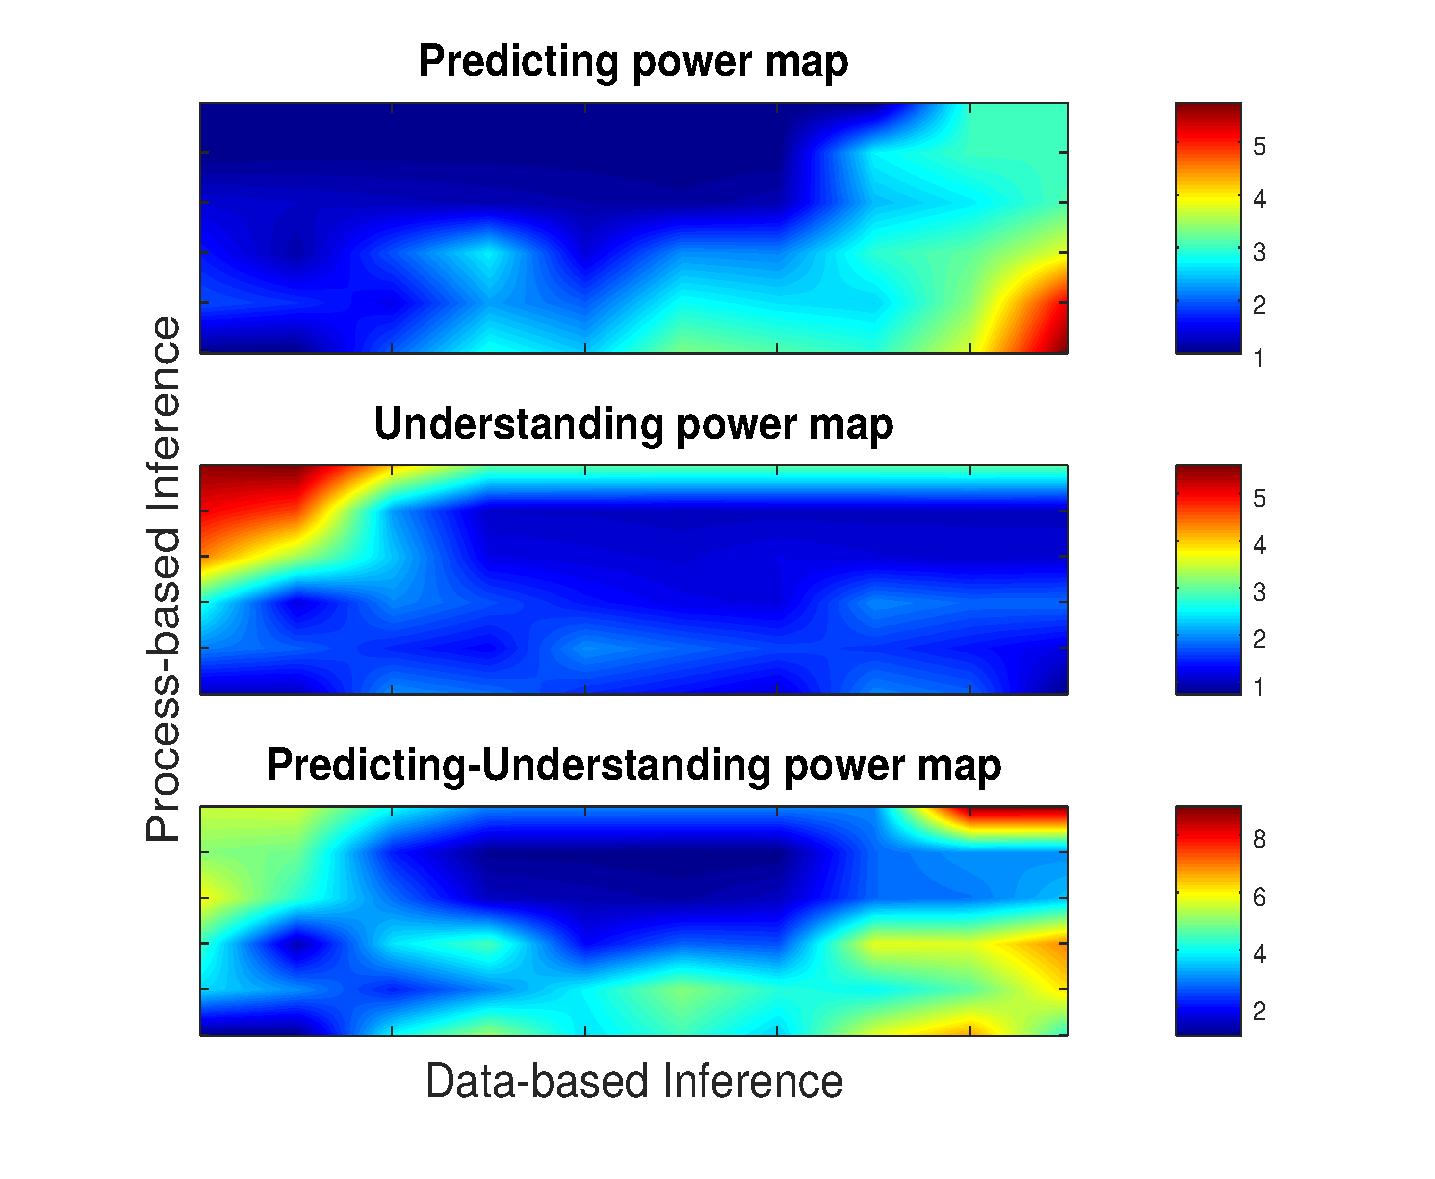
\includegraphics[width=0.85 \textwidth]{Figure3.eps}
     \end{center}
     \vspace{0.2 in}
     \caption{{\bf Figure 3: Prediction and understanding power
         map}. This figures shows a cartoon of a prediction power map
       (top), an understanding power map (middle), and a
       predicting-understanding power map (bottom). x- and y-axis
       represent data-based inference (i.e., gradient of AI methods
       from low (left) to high (right) predictive power) and
       process-based inference (i.e., gradient of process-based
       methods from low (bottom left) to high (top left) understanding
       power). The gradient of predicting power map (top) shows a hot
       spot red area in the bottom right highlighting the region where
       AI methods best predict the empirical data. The gradient of
       understanding power map (middle) shows a hot spot red area in
       the top left highlighting the region where the best mechanistic
       understanding occur. The predicting-understanding power map
       (bottom) shows the sum of the two previous maps highlighting a
       red hot spot where the best synthesis research joining
       predicting and understanding power of the empirical data might
       occur.}
         

   %\begin{wrapfigure}{l}{0.86\textwidth}
  \begin{center}
        \hspace{-0.75 in}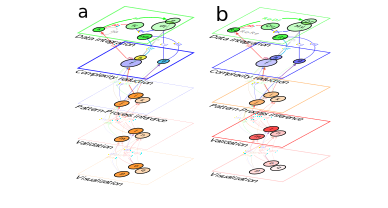
\includegraphics[width=1.05 \textwidth]{Figure4}
     \end{center}
     \vspace{-0.15 in}
     \caption{{\bf Figure 4: Prototyping a distributed and open automated research
         platform:} {\bf a)} Our initial prototype will contain five
       layers (this is not an exhaustive number. Some might be merged
       and others, like reporting generation, can be introduced): Data
       Integration, Complexity reduction, Pattern-process inference,
       Validation, and Visualization. Nodes and links represent
       algorithms and interactions between two algorithms,
       respectively. The inter-layer interactions will be implemented
       using the Renku-SDSC
       platform\footnote{\href{https://renku.readthedocs.io/en/latest/}{Renku}}. The
       intra-layer interactions will be developed initially in julia
       language (other languages will come into play during the
       development of each layer). {\bf b)} A julia-computing-language
       prototype of an automated research platform. Nodes and links in
       each layer represent julia packages and interactions between
       two packages, respectively. The figure shows the julia packages
       to be used for the Data integration layer containing the
       packages "Retriever.jl" ({\bf Re}), "Query.jl" ({\bf Qu}),
       "MySQL.jl" ({\bf My}), "SQlite.jl" ({\bf lite}), and
       "DataFrames.jl" ({\bf df}). This cartoon representing many
       intra- and inter-layer connections might be helpful to show the
       vision of the platform. For example, the path taken to solve a
       specific intra- or inter-domain (fundamental or applied)
       question can be quantified by many metrics each producing a
       distribution of automated solutions across many nodes in a
       distributed and open network, the Robhoot Open Network
       (RON). This distribution can be analyzed to quantify properties
       as robustness, reproducibility and bias of a fundamental or
       applied solution.

     }
%\end{wrapfigure}

\end{document}

     \newpage
\section{{\bf Benefits for Eawag and the Biodiversity research community}}
My sabbatical period attempts to fill two main gaps in Biodiversity
research:

1) developing a platform integrating multiple datasets into process-
and ruled-based approaches framing it in multilayer and deep learning
networks. The sabbatical will allow me to strengthen international
collaborations by submitting a FET-OPEN-EU research grant
proposal. The platform, will be fully developed in open source
software and coupled to the Renku platform (Swiss data Science Center)
and Eawag IT domain. The interactions among different platforms (i.e.,
Renku, Robhoot and others) will be a collective, multi-institutional
networking effort to integrate transdisciplinary, fundamental and
applied Biodiversity research. This will help Eawag to strengthen its
cooperatiop with international open research platforms by providing
expertise and data from Aquatic ecosystems.
\\
2) connecting fundamental and applied research combining open research
platforms can provide meaningful for enriching management forums in
applied conservation and sustainability centers. Centers that can
benefit from such tools in Switzerland and abroad will be the Wyss
Centre for Biodiversity, Climate Change and Land use with four planned
institutes worldwide, the NCCR centre in Bern and the LifeWatch EU
initiative in different parts of Europe. The CEEB could contribute to
an emerging network of Swiss synthesis centres with emphasis on
distributed and open-data-source driven biodiversity research centers
joining fundamental and applied research.
%\subsection{{\bf International host center for the sabbatical}}

%I've been discussing options for my sabbatical with complex systems
%institutes in Europe, the Amsterdam, IAS, and the Mallorca, IFISC, and
%in the USA, the New England, NECSI, and the Santa Fe Institute,
%SFI. They all have excellent teams for implementing computing
%platforms, computing facilities to run locally prototypes without much
%server regulations, together with Linux driven IT teams and team of
%researchers I would like to work with. After contrasting the pros and
%cons of each of these centers, I have chosen the one in Mallorca.

%The IFISC in Mallorca has a easy accessible full team of IT researchers
%like database and platforms developers and scientists thinking broadly
%about complex networks.


%\newpage
%\bibliographystyle{evolution}
%\bibliography{ref}
